\chapter{Architettura iniziale}
\label{cha:architettura_iniziale}

In questo capitolo viene descritto lo stato iniziale di SATAYO, la sua complessità
e i problemi di scalabilità che hanno portato alla necessità di ripensare l'architettura
del progetto.

\section{Struttura del progetto}
\label{sec:struttura}

Il progetto SATAYO è strutturato in modo tale da permettere la distribuzione del
lavoro su più macchine virtuali. In questo, dal punto di vista teorico, modo è inerentemente
più semplice scalare l'applicazione in base alla quantità e alla dimensione dei domini
che vengono analizzati dalla piattaforma.

\begin{figure}[h!]
  \centering
  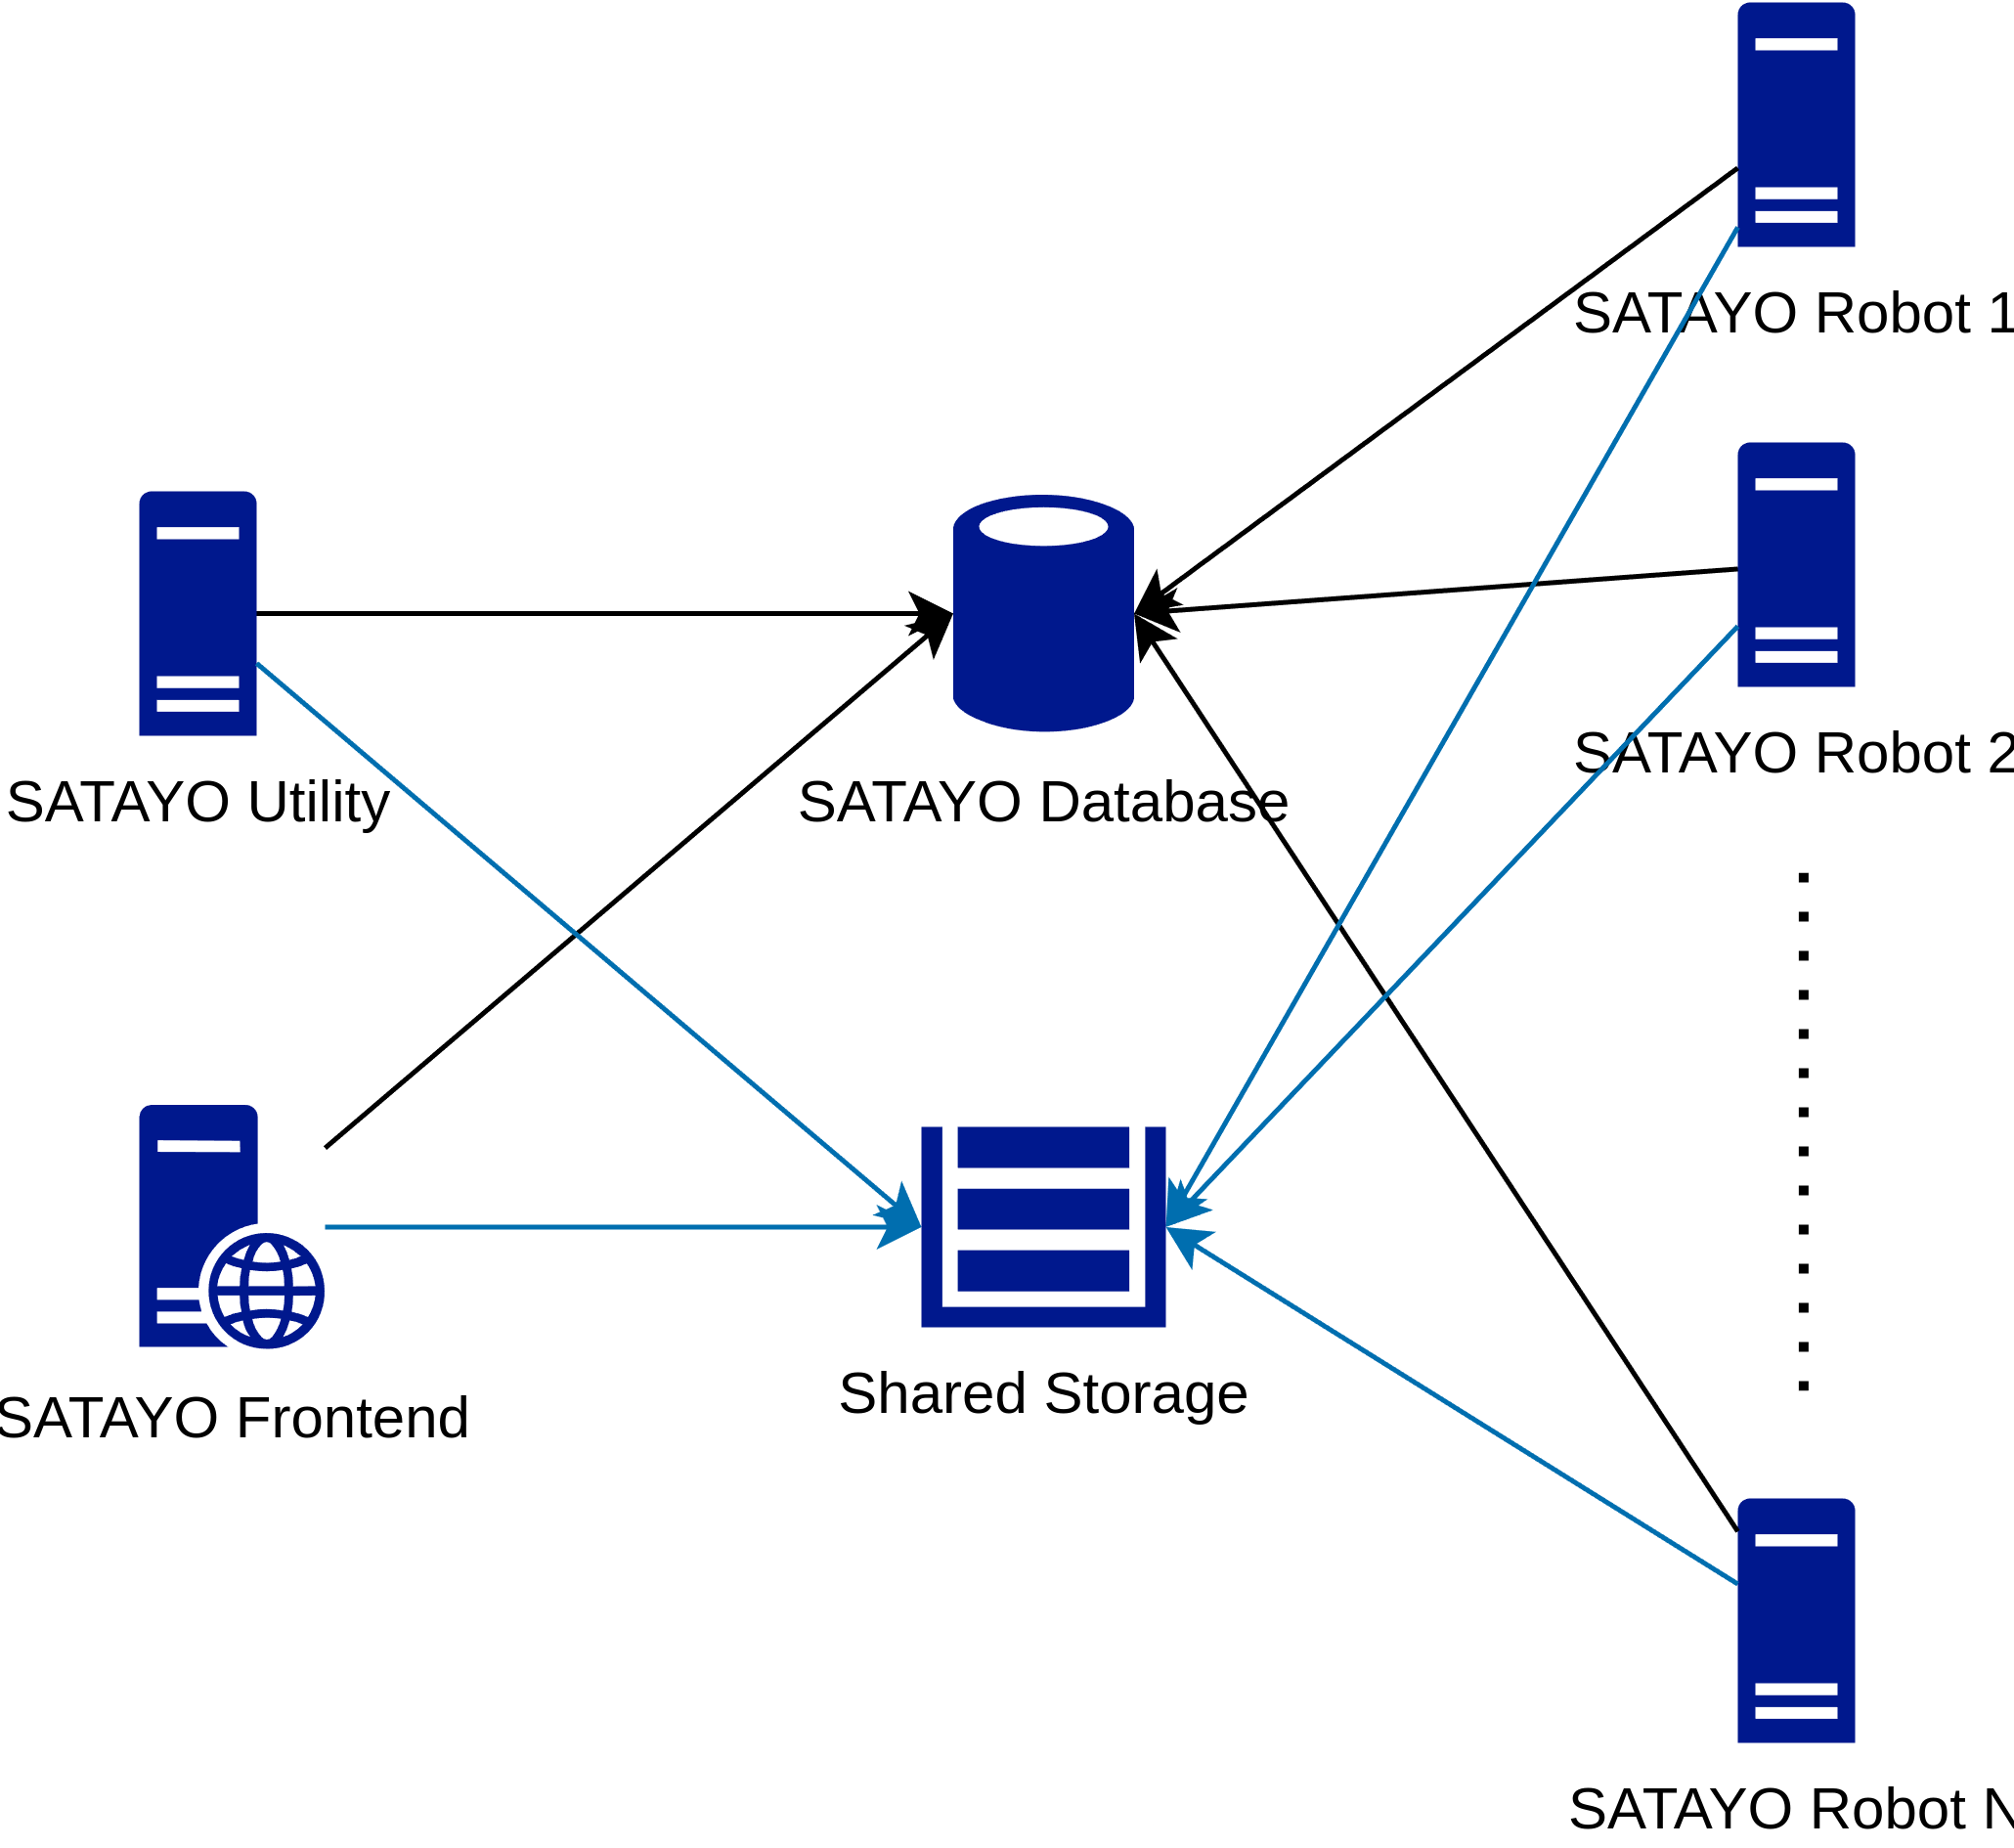
\includegraphics[width=.6\linewidth]{images/SATAYO_infrastructure_old.png}
  \caption{Vecchia infrastruttura di SATAYO}
  \label{fig:infra_old}
\end{figure}

Come si nota in figura \ref{fig:infra_old}, sono presenti tre categorie di macchine
con compiti distinti:

\begin{itemize}
  \item \textbf{SATAYO Frontend:} dedicata all'hosting del webserver con cui i
    clienti si interfacciano per utilizzare la piattaforma. Questa macchina ha la
    necessità di interfacciarsi con il database, per leggere i dati generati da
    SATAYO e per inserire nuovi domini o informazione relativi a questi nella
    piattaforma. La stessa macchina ha inoltre bisogno di permessi di lettura sullo
    storage condiviso, in cui vengono salvate le evidenze trovate sulle varie
    piattaforme OSINT da SATAYO, per presentarle agli analisti che ne devono valutare
    la correttezza e gravità;

  \item \textbf{SATAYO Utility:} la sua funzione principale è quella di eseguire
    fasi molto scalabili orizzontalmente, fasi cioè il cui tempo di esecuzione e
    carico sul sistema dipende in minima parte o non dipende affatto dal numero di
    input. Esempi specifici di queste esecuzioni possono essere lo scraping di
    siti web o di canali Telegram. Come la SATAYO Frontend anche SATAYO Utility comunica
    con il database, principalmente per inserire dati, e con lo storage condiviso
    per salvare evidenze collezionate da fonti varie;

  \item \textbf{SATAYO Robot:} argomento principale di questo elaborato, hanno il
    compito di eseguire tutte le fasi legate ad un particolare dominio.
    Generalmente si tratta di programmi e tool open-source e di terze parti che
    lavorano su input singoli, impedendo così una parallelizzazione analoga alle
    fasi Utility. Altra particolare caratteristica delle macchine Robots, che vedremo
    più nel dettaglio al punto \ref{sub:robots}, è la necessità di eseguire le
    operazioni secondo un insieme di dipendenze. Per esempio una funzione che ritorna
    una lista di servizi online a cui sono iscritti i dipendenti tramite email aziendali
    deve essere eseguita dopo la fase che si occupa di raccogliere la lista di dipendenti
    di una determinata azienda. Questa famiglia di macchine, come la SATAYO Utility,
    si interfaccia direttamente con il database e con lo storage condiviso.
\end{itemize}

In fine è presente il database, il quale è ospitato su una macchina dedicata per
poter garantire una performance migliore. Quest'ultima, analogamente allo storage
condiviso, è protetta da policy di sicurezza più strette rispetto alle altre
macchine che hanno bisogno di comunicare e interagire con la rete esterna.

\subsection{Macchine Robots}
\label{sub:robots}

\lipsum[1]

\section{Struttura database}
\label{sec:database}

\lipsum[1]

\section{Problemi con architettura corrente}
\label{sec:problemi}

\lipsum[1]